% !TeX program = xelatex
% !TEX root = PTFM.tex
\documentclass[12pt,a4paper]{report}

% ----------------------------
% PAQUETES
% ----------------------------

% Idioma, motor y tipografía
\usepackage{fontspec}
\usepackage[spanish]{babel}
\setmainfont{Times New Roman}
\newfontfamily\cambriafont{Cambria}
\newfontfamily\timesfont{Times New Roman}

% Texto
\usepackage{setspace}
\usepackage{ragged2e}
\usepackage{csquotes}
\usepackage{subfiles}

\newcommand{\thesisbodyformat}{%
	\onehalfspacing
	\justifying
	\setlength{\parindent}{0pt}
	\setlength{\parskip}{0.8em}
}

% Bibliografía
\usepackage[
backend=biber,
style=apa,
sorting=nyt,
language=spanish,
doi=true,
url=true,
isbn=false
]{biblatex}

% Matemática
\usepackage{amsmath, amssymb, amsfonts}
\usepackage{mathtools}
\usepackage{bm}
\usepackage{mathrsfs}

% Tablas
\usepackage{array}
\usepackage{booktabs}
\usepackage{longtable}
\usepackage{multirow}
\usepackage{threeparttable}
\usepackage{adjustbox}
\usepackage{tabularx}
\usepackage[table]{xcolor}
\newcolumntype{L}[1]{>{\RaggedRight\arraybackslash}p{#1}}

% Gráficos
\usepackage{graphicx}
\usepackage{pdfpages}
\usepackage{float}
\usepackage{subcaption}

% Diseño
\usepackage{geometry}
\usepackage{xcolor}
\usepackage[hang,flushmargin]{footmisc}
\usepackage[toc,page]{appendix}

% Hipervínculos
\usepackage{hyperref}
\hypersetup{
	colorlinks=true,
	linkcolor=black,
	citecolor=black,
	urlcolor=black
}


\hypersetup{
	pdfauthor={Julián Alberto Delgadillo Marín},
	pdftitle={Rentas extractivas y transformación estructural externa en economías dependientes de recursos naturales no renovables (1996–2022)},
	pdfsubject={Tesis de Maestría en Economía Aplicada},
	pdfkeywords={economic complexity, natural resources, structural transformation, diversification},
	pdfcreator={LaTeX},
	pdfproducer={XeLaTeX}
}

\usepackage{cleveref}


% Utilidades
\usepackage{etoolbox}

% Páginas por capítulo (contador interno de la tesis)
\usepackage{zref-abspage}
\usepackage{zref-user}
\usepackage{lastpage}

\makeatletter
\newcommand{\thesisstartchap}[1]{%
	\thesisbodyformat
	\zlabel{#1-start}
}

\newcommand{\thesisendchap}[1]{%
	\zlabel{#1-end}
}

\newcommand{\thesischappages}[1]{%
	\zref@ifrefundefined{#1-start}{--}{%
		\zref@ifrefundefined{#1-end}{--}{%
			\the\numexpr\zref@extract{#1-end}{abspage}-\zref@extract{#1-start}{abspage}+1\relax
		}%
	}%
}
\makeatother

% Figuras
\usepackage{tikz}
\usetikzlibrary{positioning}
\usetikzlibrary{arrows.meta, positioning, babel}

% Nombres de referencias automáticas

\addto\extraspanish{%
	\renewcommand{\tableautorefname}{Tabla}%
	\renewcommand{\figureautorefname}{Figura}%
	\renewcommand{\chapterautorefname}{Capítulo}%
	\renewcommand{\sectionautorefname}{Sección}%
	\renewcommand{\subsectionautorefname}{Subsección}%
}

% Contador pie de pagina
\makeatletter
\@removefromreset{footnote}{chapter}
\makeatother

% Jerarquía visual: Capítulos, secciones y subsecciones
\usepackage{titlesec}
\usepackage{sectsty}
\sectionfont{\raggedright}
\subsectionfont{\raggedright}

% \titleclass{\chapter}{page}

\titleformat{\chapter}
{\normalfont\huge\bfseries}
{\thechapter.}
{1em}
{}

\titlespacing*{\chapter}
{0pt}
{0pt}
{20pt}

% Secciones
\titleformat{\section}
{\centering\normalfont\bfseries\Large}
{\thesection.}
{1em}
{}

\titlespacing*{\section}
{0pt}{17pt}{10pt}

% Subsecciones
\titleformat{\subsection}[hang]
{\normalfont\large\bfseries\raggedright}
{\thesubsection.}
{1em}
{}

\titlespacing*{\subsection}
{0pt}{12pt}{6pt}

% ----------------------------
% MÁRGENES (SEGÚN NORMATIVA)
% ----------------------------
\geometry{
	left=3cm,
	right=2.5cm,
	top=2.5cm,
	bottom=2.5cm
}

% ----------------------------
% FUENTE
% ----------------------------
\setlength{\parindent}{0pt}

% ----------------------------
% COLOR Y LÍNEA (REPISA REAL)
% ----------------------------
\definecolor{lineblue}{RGB}{0,51,102}

\newcommand{\ShelfRule}{%
	\vspace{-0.15cm}
	\par\noindent
	\textcolor{lineblue}{\rule{\linewidth}{0.6pt}}%
}

% ----------------------------
% CONFIGURACIÓN BIBLIOGRAFÍA
% ----------------------------

\addbibresource{\subfix{references.bib}}

% ----------------------------
% Configuración del encabezado y numeración
% ----------------------------
\usepackage{fancyhdr}
\setlength{\headheight}{14.9pt}
\pagestyle{fancy}

% Limpia encabezados y pies
\fancyhf{}

% Encabezado (nombre del capítulo)
\fancyhead[L]{\nouppercase{\leftmark}}

% Número de página centrado en el pie
\fancyfoot[C]{\thepage}

% Sin línea superior
\renewcommand{\headrulewidth}{0pt}

% Redefinir el estilo 'plain'
% (usado en inicios de capítulo)
\fancypagestyle{plain}{
	\fancyhf{}
	\fancyfoot[C]{\thepage}
}


\begin{document}
	
	% =====================================================
	% PORTADA
	% =====================================================
	\begin{titlepage}
		
		% ----------------------------
		% INSTITUCIÓN (CAMBRIA)
		% ----------------------------
		\begin{center}
			{\cambriafont\fontsize{26}{31}\selectfont Universidad de Buenos Aires}
			
			\vspace{0.25cm}
			
			{\cambriafont\fontsize{26}{31}\selectfont Facultad de Ciencias Económicas}
			
			\vspace{0.25cm}
			
			{\cambriafont\fontsize{20}{24}\selectfont Escuela de Negocios y Administración Pública}
		\end{center}
		
		\ShelfRule
		\vspace{1.2cm}
		
		% ----------------------------
		% MAESTRÍA (CAMBRIA, NEGRITA)
		% ----------------------------
		\begin{center}
			{\cambriafont\fontsize{22}{26}\selectfont\textbf{MAESTRÍA EN ECONOMÍA APLICADA}}
		\end{center}
		
		\ShelfRule
		\vspace{1.5cm}
		
		% ----------------------------
		% TIPO DE TRABAJO (CAMBRIA)
		% ----------------------------
		\begin{center}
			{\cambriafont\fontsize{22}{26}\selectfont PROYECTO}

			\vspace{0.25cm}

			{\cambriafont\fontsize{22}{26}\selectfont TRABAJO FINAL DE MAESTRÍA}
		\end{center}
		
		\ShelfRule
		\vspace{1.5cm}
		
		% ----------------------------
		% TÍTULO DEL TFM (CAMBRIA)
		% ----------------------------
		\begin{center}
			\begin{minipage}{0.9\textwidth}
				\noindent\justifying
				{\cambriafont\fontsize{18}{22}\selectfont
					Rentas extractivas y transformación estructural externa en economías dependientes de recursos naturales no renovables (1996–2022)}
			\end{minipage}
		\end{center}
		
		\ShelfRule
		\vspace{1.8cm}
		
		% ----------------------------
		% AUTOR Y DIRECTOR (TIMES NEW ROMAN)
		% ----------------------------
		\begin{center}
			\begin{minipage}{0.9\textwidth}
				\raggedright
				{\timesfont\fontsize{14}{17}\selectfont
					\MakeUppercase{Autor: Julián Delgadillo Marín}}
				
				\vspace{0.25cm}
				
				{\timesfont\fontsize{14}{17}\selectfont
					\MakeUppercase{Director: Martín Grandes}}
			\end{minipage}
		\end{center}
		
		\vfill
		
		% ----------------------------
		% FECHA
		% ----------------------------
		\begin{center}
			{\cambriafont\fontsize{12}{14}\selectfont \MakeUppercase{\today}}
		\end{center}
		\ShelfRule
		
	\end{titlepage}
	% ====================================================
	
	% =====================================================
	% A PARTIR DE AQUÍ: TESIS (INTERLINEADO 1.5)
	% =====================================================
	\thesisbodyformat
	\pagenumbering{arabic}
	
		% =====================================================
	% DEDICATORIA (OPCIONAL)
	% =====================================================
	% \section*{Dedicatoria}
	% \label{chap:dedicatoria}
	
	% =====================================================
	% RESUMEN Y PALABRAS CLAVE
	% =====================================================
	\chapter*{Resumen}
	\label{chap:resumen}

	Esta investigación analiza por qué algunas economías dependientes de recursos naturales no renovables logran traducir las rentas extractivas en trayectorias más favorables de transformación estructural externa, mientras otras permanecen atrapadas en patrones de especialización extractiva. Para ello, el estudio distingue entre la dependencia externa de recursos, utilizada como criterio de delimitación de la muestra a partir de la estructura exportadora, y la intensidad macroeconómica de las rentas extractivas, incorporada como mecanismo explicativo dentro del modelo empírico. A partir de un diseño cuantitativo, longitudinal y comparado, basado en datos de panel para economías dependientes de petróleo, gas y minería durante el período principal 1996–2022, la investigación examina la relación entre rentas de recursos naturales, calidad institucional, condiciones macroeconómicas, capacidades productivas e innovación. La transformación estructural externa se aproxima mediante el Índice de Complejidad Económica (ECI) y, de manera complementaria, mediante la diversificación exportadora definida como $DIVX=1-HHI$. El trabajo busca aportar evidencia comparada sobre las condiciones bajo las cuales las rentas extractivas se asocian con mayores o menores niveles de sofisticación y diversificación de la canasta exportadora.

	\noindent\textbf{Palabras clave:} recursos naturales no renovables; rentas extractivas; complejidad económica; transformación estructural; diversificación exportadora.

	\section*{Abstract}
	\label{chap:abstract}

	This research examines why some economies dependent on non-renewable natural resources are able to translate extractive rents into more favorable paths of external structural transformation, while others remain locked into extractive specialization. The study distinguishes between external resource dependence, used to define the sample on the basis of export structure, and the macroeconomic intensity of extractive rents, incorporated as an explanatory mechanism in the empirical model. Using a quantitative, longitudinal, and comparative design based on panel data for oil-, gas-, and mining-dependent economies over the main estimation period 1996–2022, the research analyzes the relationship between natural resource rents, institutional quality, macroeconomic conditions, productive capabilities, and innovation. External structural transformation is proxied by the Economic Complexity Index (ECI) and, complementarily, by export diversification, defined as $DIVX=1-HHI$. The study aims to provide comparative evidence on the conditions under which extractive rents are associated with higher or lower levels of export sophistication and diversification.

	\noindent\textbf{Keywords:} non-renewable natural resources; extractive rents; economic complexity; structural transformation; export diversification.
	
	% =====================================================
	% ÍNDICE GENERAL
	% =====================================================
	\tableofcontents
	\listoffigures
	\listoftables
	
	% =====================================================
	% CUERPO DE LA TESIS
	% =====================================================
	\subfile{chapters/01-06-introduction-and-research-design/chapter.tex}
	\subfile{chapters/07-theoretical-framework/chapter.tex}
	\subfile{chapters/08-empirical-literature/chapter.tex}
	\subfile{chapters/09-methodology/chapter.tex}
	\subfile{chapters/10-data-and-variables/chapter.tex}
	\subfile{chapters/13-cronograma/cronograma.tex}
	\subfile{chapters/bibliography/bibliography.tex}
	\subfile{chapters/appendices/appendices.tex}
	\clearpage
	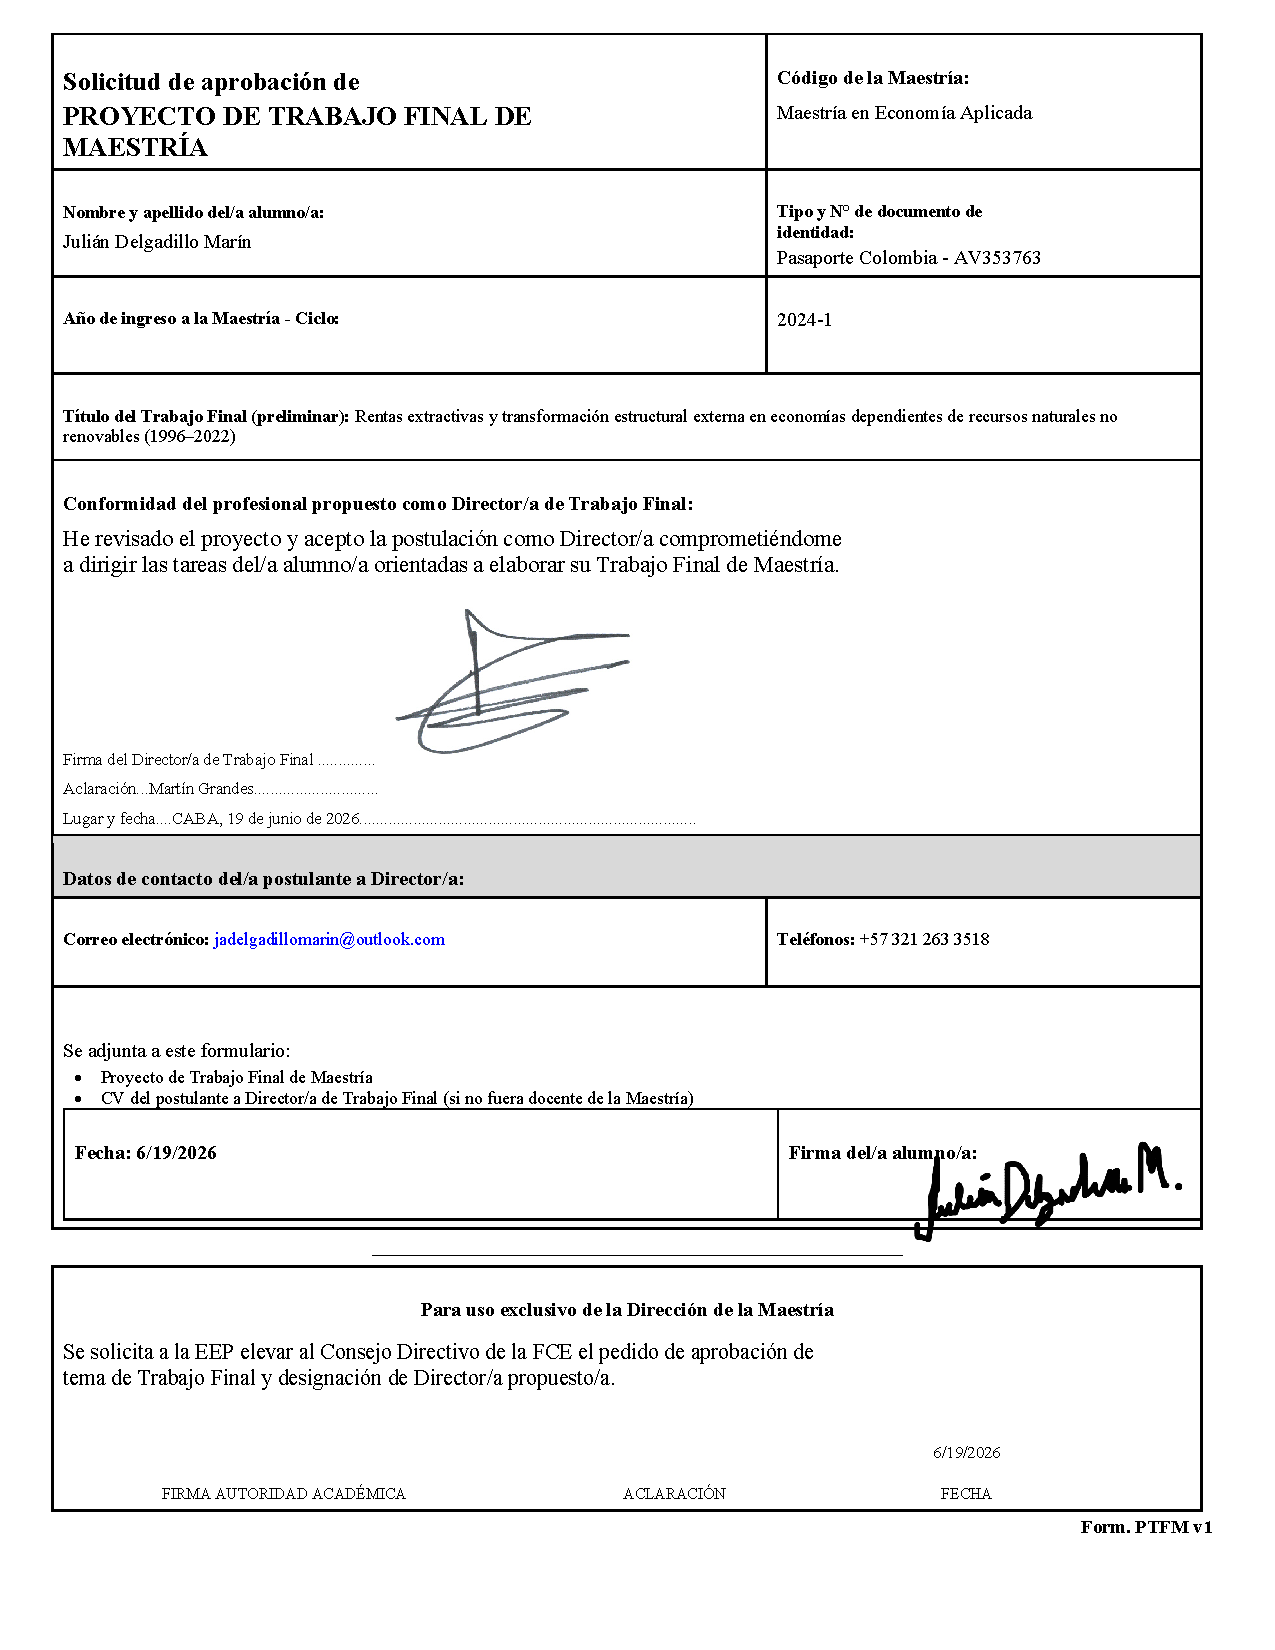
\includepdf[
		pages=-,
		pagecommand={\thispagestyle{empty}},
		fitpaper=true
	]{chapters/14-approval-form/approval-form-director.pdf}
	
\end{document}
